\section{eplusscreen.csv}\label{eplusscreen.csv}

Results of the window screen transmittance map. This file can be used to create a 3-D Column chart for graphically viewing the direct beam and reflected beam transmittance at various relative azimuth and relative altitude angles. The ``relative'' angles in this file are the incident solar angles with respect to the outward surface normal. The figures below are example 3-D charts generated using the data provided in this output file.

\begin{figure}[htbp]
\centering
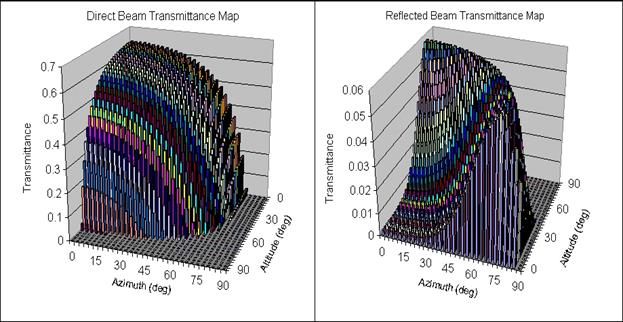
\includegraphics{media/image022.jpg}
\caption{TransmittancePlotExample}
\end{figure}
